%% LaTeX-Beamer template for KIT design
%% by Erik Burger, Christian Hammer
%% title picture by Klaus Krogmann
%%
%% version 2.1
%%
%% mostly compatible to KIT corporate design v2.0
%% http://intranet.kit.edu/gestaltungsrichtlinien.php
%%
%% Problems, bugs and comments to
%% burger@kit.edu

\documentclass[18pt]{beamer}

%% SLIDE FORMAT

% use 'beamerthemekit' for standard 4:3 ratio
% for widescreen slides (16:9), use 'beamerthemekitwide'


\usepackage{templates/beamerthemekit}
% \usepackage{templates/beamerthemekitwide}

%% TITLE PICTURE

% if a custom picture is to be used on the title page, copy it into the 'logos'
% directory, in the line below, replace 'mypicture' with the 
% filename (without extension) and uncomment the following line
% (picture proportions: 63 : 20 for standard, 169 : 40 for wide
% *.eps format if you use latex+dvips+ps2pdf, 
% *.jpg/*.png/*.pdf if you use pdflatex)

%% Define some colors:
\definecolor{darkblue}{rgb}{0,0,.5}
\definecolor{darkgreen}{rgb}{0,.5,0}

\titleimage{banner}

%% TITLE LOGO

% for a custom logo on the front page, copy your file into the 'logos'
% directory, insert the filename in the line below and uncomment it

\titlelogo{logo_150x150}

% (*.eps format if you use latex+dvips+ps2pdf,
% *.jpg/*.png/*.pdf if you use pdflatex)

%% TikZ INTEGRATION

% use these packages for PCM symbols and UML classes
% \usepackage{templates/tikzkit}
% \usepackage{templates/tikzuml}

% the presentation starts here

\title[Tutorium 2]{GBI Tutorium Nr. 32}
\subtitle{Tutorium 2}
\author{Dominik Muth - dominik.muth@student.kit.edu}

\institute{Institut f\"ur Informatik}

% Bibliography

\usepackage[citestyle=authoryear,bibstyle=numeric,hyperref,backend=biber]{biblatex}
\addbibresource{templates/example.bib}
\bibhang1em

\begin{document}

	% change the following line to "ngerman" for German style date and logos
	\selectlanguage{ngerman}

	%title page
	\begin{frame}
		\titlepage
	\end{frame}

	%table of contents
	\begin{frame}{Outline/Gliederung}
		\tableofcontents
	\end{frame}
	
	
	\section{\"Ubungsblatt 1}
	\begin{frame} {\"Ubungsblatt 1}
		\begin{block} {Aufgabe 1.2}
			Gegeben seien zwei beliebige, nichtleere, endliche Mengen A und B, sowie eine injektive Abbildung $f: A \rightarrow B$.\\
			\vspace{10pt}
			b) Geben Sie eine surjektive Abbildung $g: B \rightarrow A$ an.
		\end{block}
		\begin{overprint}
			\onslide<2> $g(x) = f(x)^{-1}$ ?
			\onslide<3-5> \color{red} $g(x) = f(x)^{-1}$ !\\
			
		\end{overprint}
		\begin{overprint}
			\onslide<4> $g(x) = \left\{\begin{array}{ll} a & , falls$ $f(a) = x\\
         a' & , sonst\end{array}\right. .$
			\onslide<5> \color{darkgreen}$g(x) = \left\{\begin{array}{ll} a & , falls$ $f(a) = x\\
         a' & , sonst\end{array}\right. .$
		\end{overprint}
	
	\end{frame}		
	
	\section{Wiederholung} 
	\begin{frame} {Wiederholung}
		\begin{itemize}
		\item $f(x) = x + 1$ mit $x \in \mathbb{N}$ und $f(x) \in \mathbb{N}$ ist surjektiv.\\
		\visible<2-4> {\color{red} falsch\\}
			\vspace{10pt}
		\color{black}
		\item $A \times B$ ist eine Relation.\\
		\visible<3-4> {\color{darkgreen} richtig\\}
			\vspace{10pt}
		\color{black}\item 
		Eine Rechtstotale und Linkseindeutige Relation nennt man auch Abbildung/Funktion.\\
		\visible<4> {\color{red} falsch\\}
		
		\end{itemize}
	\end{frame}
	
	\section{Aussagenlogik}
	\begin{frame}{Aussagenlogik\\ - Logische Aussagen 1}
	Einfache Logische Aussagen:
		\begin{itemize}
			\item Negation $\neg$A: "nicht A"
			\pause
			\item Logisches Und (A $\land$ B): ''A und B"
			\pause
			\item Logisches Oder (A $\lor$ B): ''A oder B"
		\end{itemize}
	\end{frame}


	\begin{frame}{Aufgabenteil 1}
		\begin{block}{Aufgabe 1}
			Stelle die Wahrheitstabelle auf:\\
			$(\neg A \land B) \lor \neg B$
		\end{block}
		
		\begin{block}{Aufgabe 2}
			Stelle die Wahrheitstabelle auf:\\
			$(A \land B \land \neg C) \lor (C \land A) \lor (C \land B)$
		\end{block}
	\end{frame}


	\begin{frame}{Aussagenlogik\\ - Logische Aussagen 2}
		\begin{itemize}
			\item Implikation (A $\Rightarrow$ B): "Wenn A, dann B"
			\pause
			\item \"Aquivalenz (A $\Leftrightarrow$ B): ''A genau dann, wenn B" (Implikation in beide Richtungen)
		\end{itemize}
	\end{frame}


	\begin{frame}{Aufgabenteil 2}
		\begin{block}{Aufgabe 1}
			Stelle die Wahrheitstabelle auf:\\
			$(A \Rightarrow B) \Rightarrow C$
		\end{block}
		
		\begin{block}{Aufgabe 2}
			Sind die Beiden Aussagen \"Aquivalent?:\\
			$\neg (A \Rightarrow B) \Leftrightarrow \neg (\neg A \lor B)$
		\end{block}
	\end{frame}
	
	
	\section{W\"orter}
	\begin{frame} {W\"orter}
		\begin{block} {Definition}
			Ein Wort ist eine Folge an Zeichen aus einem Alphabet $A$.\\
			Wobei ein Alphabet eine nichtlehre Menge an Zeichen ist.
		\end{block}
		
		\pause
	
		\begin{exampleblock} {Beispiel}
			\begin{itemize}
				\item $A = \left\{H, a, l, o, \textvisiblespace, W, e, t\right\}$  enth\"alt das Wort\\
            Hallo Welt
            \pause
            \item Hallo Welt $\in \mathbb{G}_{10} \rightarrow A = A^{10}$
            \pause
            \item $\Rightarrow$ die Relation $\mathbb{G}_{10} \rightarrow A$ enth\"allt alle W\"orter der L\"ange 10, welche mit dem Alphabet A gebildet werden können. 
			\end{itemize}
	
		\end{exampleblock}
	\end{frame}
	
	
	\begin{frame} {Menge aller W\"orter}
		\begin{block} {Definition}
			Die Menge aller W\"orter \"uber einem Alphabet $A$ sind alle W\"orter, in denen nur Zeichen aus $A$ enthalten sind. Dies wird als $A^*$ geschrieben.
		\end{block}
		\pause
		\begin{exampleblock} {Beispiel}
			Gegeben sei das Alphabet $A = \{a, b\}$, dann enth\"alt A*: \\
			\begin{itemize}
				\item $\epsilon$ (Das leere Wort)
				\item a
				\item b
				\item aa
				\item ab
				\item ba
				\item \dots
			\end{itemize}
		\end{exampleblock}
	\end{frame}
	
	
	\begin{frame} {Das leere Wort $\epsilon$}
		\begin{block} {Definition}
			Das leere Wort ($\epsilon$) bezeichnet ein Wort ohne Inhalt und hat die L\"ange 0.\\
			Aus der L\"ange von $\epsilon$ folgt, dass $\epsilon \not= Leerzeichen$, da das Leerzeichen die L\"ange 1 hat.		
		\end{block}
	\end{frame}
	
	
	\begin{frame} {Konkatenation von W\"ortern}
		\begin{block} {Definition}
			Eine Konkatenation von W\"ortern ist das zusammensetzten dieser W\"orter.\\
			Formal: $\omega_1 \cdot \omega_2$
		\end{block}
		
		\pause		
		
		\begin{exampleblock} {Beispiel}
			\begin{itemize}
				\item $A = \{K, l, e\}$ enth\"allt das Wort $\omega_1 = Klee$
				\item $B = \{b, l, a, t\}$ enth\"allt das Wort $\omega_2 = blatt$
				\pause
				\item $\omega_1 \cdot \omega_2 = Kleeblatt \not= \omega_2 \cdot \omega_1 = blattKlee$
				\pause
				\item $\omega_1 \cdot \epsilon \cdot \omega_2 = Kleeblatt$
			\end{itemize}
		\end{exampleblock}
	\end{frame}
	
	
	\begin{frame} {Potenzen von W\"ortern}
		\begin{exampleblock} {Beispiel}
			\begin{itemize}
				\item $\omega = ha$
				\item $\omega^2 = haha$
				\item $\omega^3 = hahaha$
			\end{itemize}
		\end{exampleblock}
	\end{frame}
	
	
	\begin{frame} {Aufgabenteil 3}
		\begin{itemize}
			\item was ist $a^k$, was ist $b^k$ ?
			\pause
			\item was ist $a^kb^k$ ?
			\pause
			\item was ist $(ab)^k$ ?
		\end{itemize}
	\end{frame}
	
	
	\begin{frame} {Wortl\"ange}
		\begin{block} {Definition}
			Die L\"ange eines Wortes $\omega$ gibt die Anzahl der darin enthaltenen Zeichen an. \\
			Formal: $|\omega|$
		\end{block}
		
		\begin{exampleblock} {Beispiel}
			\begin{itemize}
				\item $|Hallo Welt| = 10$
				\pause
				\item $|\omega^k| = k \cdot |\omega|$
				\pause
				\item $|\epsilon| = 0$
				\pause
				\item $|\omega_1 \cdot \omega_2| = |\omega_1| + |\omega_2|$
			\end{itemize}
		\end{exampleblock}
	\end{frame}
	
	
	\section{Vollst\"andige Induktion}
	\begin{frame} {Vollst\"andige Induktion}
		\begin{block} {Definition}
			Die vollst\"andige Induktion ist ein Mathematisches bewei\ss{}verfahren.\\
		\end{block}
		
		\begin{exampleblock} {Struktur}
			\begin{itemize}
				\item Induktionsanfang (IA)
				\item Induktionsvoraussetzung (IV)
				\item Induktionsschluss / Induktionsschritt (IS)
			\end{itemize}
		\end{exampleblock}
	\end{frame}
	
	\begin{frame} {Funktionsweise}
		\begin{itemize}
			\item IA: wir beweisen, dass das Problem f\"ur das kleinst m\"ogliche $n$ g\"ultig ist.
			\pause
			\item IV: Wir nehmen an, dass wenn das Problem f\"ur $n$ g\"ultig ist, dass es ebenso f\"ur $n+1$ g\"ultig ist.
			\pause
			\item IS: Wir beweisen, dass wenn wir f\"ur $n$, $n+1$ einsetzten das Problem g\"ultig ist.
		\end{itemize}
	\end{frame}
	
	
	\begin{frame} {Beispiel Vollst\"andige Induktion}
		\begin{block}{}
			$\forall n \in \mathbb{N}_+ : n^3 + 5n$ ist durch 6 teilbar.
		\end{block}
		
		\begin{block}{}
			\begin{itemize}
				\item IA: F\"ur $n = 1$: $1^3 + 5 = 6$ $\surd$
				\pause
				\item IV: F\"ur alle $\forall n \in \mathbb{N}_+$ gelte, $n^3 + 5n$ sei durch 6 teilbar.
				\pause
				\item IS: F\"ur $n = n+1$: \\
				 $(n+1)^3 + 5(n+1)$\\
				\pause
				 $=n^3 + 3n^2 + 3n + 1 + 5n + 5$\\
				\pause
				 $=(n^3 + 5n) + 3n(n+1) + 6$\\
				\pause
				 $\Rightarrow IV + 3(n^2+n+2)$ $\surd$\\
				 Da $3*(n^2+n+2)$ immer ein gerades vielfaches von 3 ist.
			\end{itemize}
		\end{block}
	\end{frame}
	
	
	\begin{frame} {Aufgabenteil 4}
		\begin{block} {}
			Zeigen Sie durch vollst\"andige Induktion:\\
			\vspace{10pt}
			$\forall n \in \mathbb{N}_+$:$2^{2n+3}+2\cdot5^{2n-1}$ ist durch 42 teilbar.
		\end{block}
	\end{frame}
	
	\section{Fragen}
	\begin{frame} {Fragen}
		\begin{itemize}
			\item Fragen zum Stoff?
			\item Fragen zum n\"achsten \"Ubungsblatt?
			\item Generelle Fragen?
		\end{itemize}
	\end{frame}

	
	\begin{frame} {EOF}
		\begin{center}
			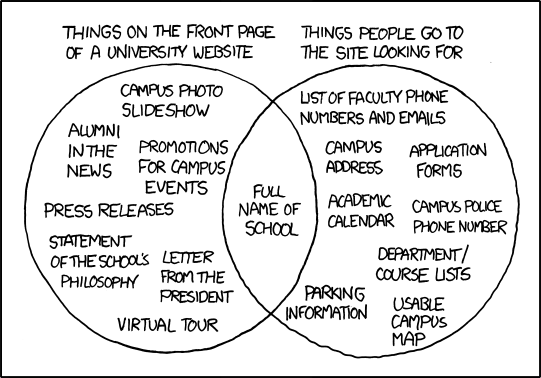
\includegraphics[scale=0.5]{graphics/02/eof2.png}\\
			\tiny source: http://imgs.xkcd.com/comics/university_website.png
		\end{center}
	\end{frame}

\end{document}
